%% A simple template for a lab or course report using the Hagenberg setup
%% based on the standard LaTeX 'report' class
%%% äöüÄÖÜß  <-- no German umlauts here? Use an UTF-8 compatible editor!

%%% Magic comments for setting the correct parameters in compatible IDEs
% !TeX encoding = utf8
% !TeX program = pdflatex 
% !TeX spellcheck = en_US
% !BIB program = biber

\documentclass[english,notitlepage,smartquotes]{hgbreport}
% Valid options in [..]: 
%    Main language: 'german' (default), 'english'
%    Turn on smart quote handling: 'smartquotes'
%    APA bibliography style: 'apa'
%    Do not create a separate title page: 'notitlepage'
%%%-----------------------------------------------------------------------------

\RequirePackage[utf8]{inputenc} % Remove when using lualatex or xelatex!

\renewcommand{\chapter}[1]{} % Disable \chapter command
\graphicspath{{images/}}     % Location of images and graphics
\bibliography{references}    % Biblatex bibliography file (references.bib)
\ExecuteBibliographyOptions{backref=false} % No back references in bibliography

%%%-----------------------------------------------------------------------------
\setcounter{chapter}{1}	% <----- set to assignment number!
%%%-----------------------------------------------------------------------------

\author{Julian Emanuel Jany}                     % Your name
\title{Evaluation and identification of the optimization potential of modern demosaicing algorithms \\ % Name of the course
			 Exposé}
\date{\today}

%%%-----------------------------------------------------------------------------
\begin{document}
%%%-----------------------------------------------------------------------------
\maketitle
%%%-----------------------------------------------------------------------------

% \begin{abstract}\noindent
% This lab unit deals with various interesting problems \ldots (give a short
% summary of the specific topics addressed). If you decide to write your report in
% German, make sure to change the \verb!\documentclass! parameter from
% \texttt{english} to \texttt{german}.
% If you write in MS Word (and such), try to use a similar structure.
% \end{abstract}

%%%-----------------------------------------------------------------------------

\section{Motivation}

The majority of imaging devices utilize only a single image sensor. This inherently results in a one-dimensional signal. To enable mutli-spectral imaging a Color Filter Array (CFA) is placed on top of the sensor array. Typically the CFA is implemented as a repeating pattern of three different filters. The most popular CFA is the Bayer CFA (see Fig. \ref{fig:bayer_cfa}).

\begin{figure}[]
	\centering
	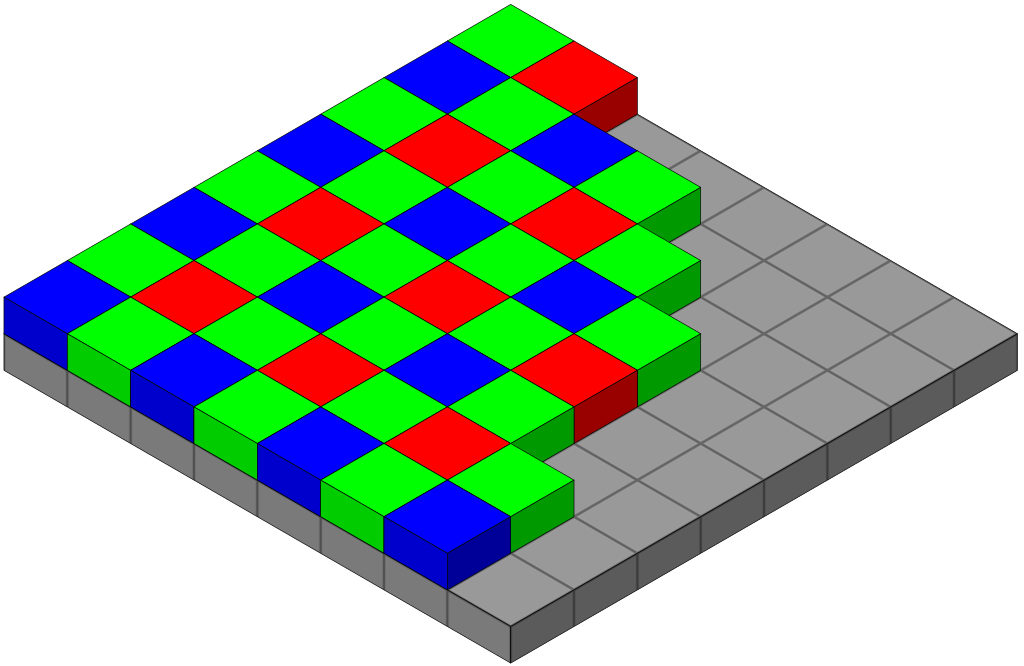
\includegraphics[width=0.35\textwidth]{bayer_pattern}
\caption{Image sensor array partially covered by a Bayer CFA. \cite{BayerCFA}}
\label{fig:bayer_cfa}
\end{figure}

Demosaicing is the process of reconstructing the two missing color channel signals for every sensel to form a "full color" image. This is usually one of the first stages of a digital imaging pipeline and has a significant influence on the quality of the final image.

\section{Objectives} % "Ziele"

\section{Tasks}

\section{Research Questions}

\section{Organizational Details}

The master thesis is written in English.
There is no intention to block publication of the master thesis.

\section{Milestones}

\subsection{Table of Contents}

The table of contents is handed in by \textbf{January 20, 2023} at the latest.

\subsection{Sample Chapter}

The sample chapter is handed in by \textbf{March 17, 2023} at the latest.

\subsection{Bibliography}

The bibliography is handed in by \textbf{April 28, 2023} at the latest.

\subsection{Preliminary Thesis}

The preliminary thesis is handed in by \textbf{May 29, 2023} at the latest.

\subsection{Final Thesis}

The final thesis is handed in by \textbf{June 26, 2023} at the latest.

\section{Relevant Literature}

Mittal et al. 2013 \cite{Mittal2013} introduced a blind image quality assessment model. Unlike the quality metrics commonly used to compare demosaicing algorithms -- such as the Color Peak Signal-to-Noise Ratio (CPSNR) \cite{Menon2011} -- the proposed Natural Image Quality Evaluator (NIQE) does not require full-color reference images. NIQE can be used to evaluate the demosaicing quality for full-resolution images for which no full-color reference image exists. This is the case for all photos taken with consumer cameras, since the JPEG output of the camera or raw-processor itself inherently contains demosaicing artifacts.

Menon et al. 2011 \cite{Menon2011} provide a comprehensive overview of classical demosaicing approaches.

Gharbi et al. 2016 \cite{Gharbi2016} were the first to apply a data-driven approach on the demosaicing problem. They used convolutional neural networks trained on "real" images to restore the missing data. The proposed approach showed qualitative improvements over the state-of-the-art on a variety of test sample sets. Additionally, they have shown that the traditional approach of separating demosaicing and denoising as sequential steps in the image processing pipeline is suboptimal.

Ronneberger et al. 2015 \cite{Ronneberger2015} proposed the U-Net for biomedical image segmentation. The network architecture has since produced great results in various different domains. An adapted U-Net is a promising candidate for one of the prototypes.

Kim et al. 2020 \cite{Kim2020} demonstrate an ingenious demosaicing algorithm that builds on prior work in multiple fields. Their approach delivers outstanding results for the challenging Quad Bayer CFA.

%%%-----------------------------------------------------------------------------
  
\section*{References}

\printbibliography[heading=noheader]

%%%-----------------------------------------------------------------------------
\end{document}
%%%-----------------------------------------------------------------------------
